\section*{Introduction}\label{sec:intro}
In this report we present an implementation of a Particle Filter in
C++. Before discussing the actual implementation we give the
theoretical details of the method in this section. We start by giving
a brief overview of the method before discussing the individual steps
in more detail.

We remark here, that the naming in these methods is highly ambiguous
and varies greatly from author to author and even in different
publications of the same authors. We use -- with some exceptions --
the naming and notation used in~\cite{doucet} and highlight parts
where the naming differs from other publications.

\subsection*{Overview of a Particle Filter}
A Particle Filter is a Sequential Monte Carlo (SMC)
method\footnote{Some authors use the terms \emph{Particle Filter} and
  \emph{SMC method} synonymously. Doucet and Johansen develop
  in~\cite{doucet} a framework in which Particle Filters are only one
  specific method in the much broader class of SMC methods. They argue
  that this distinction allows for a better understanding of these
  methods. In this report, we are only interested in the
  \emph{filtering problem} and we will introduce it without discussing
  the more general notion of SMC methods as given by Doucet and
  Johansen.} that is used to estimate the state of a system that
changes over time using only noisy and/ or partial observations of the
system's state. This will be done in a Bayesian framework where one
attempts to construct the posterior probability density function (pdf)
of the state based on the observations. We make the following
assumptions:
\begin{enumerate}[label=(A\arabic*)]
\item The model describing the initial state and the evolution of the
  internal state in time is available in a probablistic form.
\item The model that relates the observations to the internal state is
  available in a probabilistic form.
\item The observations are only available sequentially, not as a batch
  (ie. we assume that we receive new measurments sequentially in
  time).
\end{enumerate}
Due to (A3) we aim at a recursive method that does neither require to
store nor to reprocess all the previous information when a new
observation becomes available. To formalise the first two assumptions
we will use the notion of \emph{hidden markov models}.

Such models consist of the triplet
\begin{align*}
  \label{eq:hmm:1}
  X_0 &\sim \mu(x_0)\,,\\
  X_n \mid (X_{n-1} = x_{n-1}) &\sim p(x_n \mid x_{n-1})\,,\\
  Y_n \mid (X_n = x_n) &c\sim p(y_n \mid x_n) \,,
\end{align*}
where
\begin{itemize}
\item $n \in \N$ denotes discrete time;
\item $X_n$ is the $d_x$-dimensional state of the system taking values
  in $\R^{d_x}$;
\item $p(x_0)$ is the prior probability density fumction (pdf) of the
  system's state;\footnote{ With abuse of notation we denote by $p(x)$
    the pdf of the random variable $X$. For two random variables $X$
    and $Y$ the corresponding (possibly different) density functions
    are denoted by $p(x)$ and $p(y)$ respectively; $p(x,y)$ denotes
    the joint pdf and $p(x \mid y)$ is the conditional pdf of $X$
    given $Y = y$.}
\item $Y_n$ is the $d_y$-dimensional vector of observations which is
  assumed to be conditionally iindependent of all other observations
  given the state $X_n$,
\item $p(y_n \mid x_n)$ is the conditional pdf of $Y_n$ given
  $X_n = x_n$.
\end{itemize}
Assumptions (A1) and (A2) then state that all these pdfs are known.
Our goal is now to estimate the distribution $p(x_n \mid y_{1:n})$,
where $y_{1:n} \coloneqq (y_1, y_2, \dotsc, y_n)$. This is often
referred to as the \emph{filtering problem} or
\emph{tracking}.\footnote{Note that Docuet and Johansen \emph{do not}
  call this the filtering problem~\cite{doucet}. They reserve this
  term for the estimation of the joint distributions
  $p(x_{1:n} \mid y_{1:n} )$. Since we are only concerned with
  estimating the marginal distribution $p(x_n \mid y_{1:n} )$ we will
  still refer to this problem as filtering.}

% In principle, this is could be done in two steps: prediction and
% update. By the Chapman-Kolmogorov equation we first obtain
% \begin{align*}
%   p(x_{k+1} \mid y_{1:k}) &= \int p(x_{k+1} \mid x_k, y_{1:k}) p(x_k \mid y_{1:k}) \dx_k \\
%                           &= \int f(x_{k+1} \mid x_k) p(x_k \mid y_{1:k}) \dx_k \,,
% \end{align*}
% where we used the Markov property of the system, \ie
% \[
%   p(x_{k+1} \mid x_k, y_{1:k}) = p(x_{k+1} \mid x_k) = f(x_{k+1}
%   \mid x_k) \,.
% \]
% Once a new observation $y_{k+1}$ becomes available we can update our
% beliefs about the system's state using Bayes' theorem
% \[
%   p(x_{k+1} \mid y_{1:k+1}) = \frac{ p(y_{k+1} \mid x_{k+1})
%   p(x_{k+1} \mid y_{1:k}) }{ p(y_{k+1} \mid y_{1:k}) }\,,
% \]
% where the normalising constant
% \begin{align*}
%   p(y_{k+1} \mid y_{1:k}) &= \int p(y_{k+1} \mid x_{k+1}) p(x_{k+1} \mid y_{1:k}) \dx_{k+1} \\
%                           &= \int g(y_{k+1} \mid x_{k+1}) p(x_{k+1} \mid y_{1:k}) \dx_{k+1}
% \end{align*}
% depends on the likelihood function defined by the model
% in~\eqref{eq:hmm:2}. Putting these two steps together, we obtain a
% recursive formula using the previous filtered state of the system
% $p(x_{k} \mid y_{1:k})$ and a new observation $y_{k+1}$ to compute
% the current state of the system.
\todo{1-step-predictor (Chapman-Kolmogorov)}
In a restrictive set of cases this distribution can be computed
exactly (\eg when $p(y_t \mid y_t)$ is linear and the posterior of the
system is Gaussian~\cite[175]{arulampalam} or when the underlying
state space of the Markov model is finite, cf.~\cite[Example
1]{doucet}). In a more general nonlinear non-Gaussian setting,
approximative methods such as particle filters are
necessary. Therefore, in practice a different approach is used.

\section*{(Sequential) importance sampling}
The central idea of Particle filters is to represent the posterior of
the system $p(x_k \mid y_{1:k})$ at some time $k$ as a weighted set of
samples, so called \texttt{particles}, denoted by
$\{ x^{(i)}_k, w^{(i)}_k \}.$ If we ignore for a moment the weights
and assume that the samples are from the desired distribution, \ie
\[
  x^{(i)}_k \sim p(x_k^{(i)} \mid y_{1:k}), \quad i = 1, \dotsc, N
\]
the Monte carlo method approximates $p(x_k \mid y_{1:k})$ by the
empirical measure\footnote{Again, we slightly abuse the notation for
  simplicity; the alternations required for a rigorous
  measure-theoretic formulation are straightforward.}
\begin{equation}
  \label{eq:empirical_measure}
  \hat{p}(x_k \mid y_{1:k}) = \frac{1}{N} \sum_{i = 1}^N
  \delta_{x_k^{(i)}}(x_k)\,,
\end{equation}
where $\delta_x(\cdot)$ denotes the Dirac delta centered at $x$. The
expectation of a test function $f : \R^{d_x} \rightarrow \R$ given by
\[
  \mathbb{E}[f(x_k) \mid y_{1:k}] = \int f(x_k) p(x_k \mid y_{1_k})
  \dx_k
\]
is then estimated by
\[
  {\mathbb{E}}^{\text{MC}}[f(x_k) \mid y_{1:k}] = \int f(x_k)
  \hat{p}(x_k \mid y_{1_k}) \dx_k = \frac{1}{N} \sum_{i=1}^N
  f(x^{(i)}_k)\,.
\]
It is well-known that the variance of the approximation error using
this estimator decreases \emph{independent of $d_x$} with a rate of
$\mathcal{O}(N^{-1})$. However, often it is either impossible or
practically intractable to sample from the posterior directly and
thus, in practice one often relies on a technique called
\emph{importance sampling}.

We start by choosing an \emph{importance density}
$q(x_k \mid y_{1:k})$ and draw $N$ samples $x^{(i)}_k$ from it. If we
would use these samples to approximate $p(x_k \mid y_{1:k})$ as
in~\eqref{eq:empirical_measure} the result would obviously not be
accurate in general. To correct this bias we introduce
\emph{importance weights}
\begin{equation}
  \label{eq:importance_weights}
  w_k^{(i)} \propto \frac{p(x_k^{(i)} \mid y_{1:k})}{q(x_k^{(i)} \mid
    y_{1:k})} \,,
\end{equation}
that we require to be normalised such that $\sum_i w_k^{(i)} = 1$. We
can now approximate the target density by
\begin{equation}
  \label{eq:karget:approx}
  p(x_k \mid y_{1:k}) \approx \sum_{i=1}^N w_k^{(i)} \delta_{x_k^{(i)}}(x_k) \,.
\end{equation}
This technique is called \emph{importance sampling}. Expectations of
test functions can then be estimated by
\[
  \mathbb{E}^{\text{MC}}[f(x_k) \mid y_{1:k}] = \sum_{i=1}^N
  w_k^{(i)}f(x_k^{(i)}) \,.
\]
Due to assumption (A3) ideally we would like a recursive formula to
update the weights a each step. To obtain such a formula we consider
the full posterior $p(x_{0:k} \mid y_{1_k})$ and express it in terms
of the posterior at the previous time step and the known pdf's
$p(y_k \mid x_k)$ and $p(x_k \mid x_{k-1})$:
\begin{align*}
  p(x_{0:k} \mid y_{1:k}) &\propto p(y_k \mid x_{0:k}, y_{1:k-1}) p(x_{0:k} \mid y_{1:k-1}) \\
                          &= p(y_k \mid x_k) p(x_k \mid x_{0:k-1}, y_{1:k-1}) p(x_{0:k-1} \mid y_{1:k-1}) \\
                          &= p(y_k \mid x_k) p(x_k \mid x_{k-1}) p(x_{0:k-1} \mid y_{1:k-1})\,,
\end{align*}
where we used Bayes' theorem and the properties of the system
described earlier. If in addition we choose an importance density that
factorizes such that
\[
  q(x_{0:k} \mid y_{1:k}) = q(x_k \mid x_{0:k-1}, y_{1:k}) q(x_{0:k-1}
  \mid y_{1:k-1})
\]
the weights~\eqref{eq:importance_weights} can be written as
\begin{align*}
  w_k^{(i)} &\propto \frac{p(y_k \mid x_k^{(i)}) p(x_k^{(i)} \mid x_{k-1}^{(i)}) p(x_{0:k-1}^{(i)} \mid y_{1:k-1})}{q(x_k^{(i)} \mid x_{0:k-1}^{(i)}, y_{1:k}) q(x_{0:k-1}^{(i)} \mid y_{1:k-1})} \\
            &= \frac{p(y_k \mid x_k^{(i)}) p(x_k^{(i)} \mid x_{k-1}^{(i)})}{q(x_k^{(i)} \mid x_{0:k-1}^{(i)}, y_{1:k})} w^{(i-1)}_k \,.
\end{align*}
Since in our case, we are only interested in estimating the filtered
posterior $p(x_k \mid y_{1:k})$ we choose an importance density
$q(x_k \mid x_{0:k-1}, y_{1:k}) = q(x_k \mid x_{k-1}, y_{k})$ that
only depends on $x_{k-1}$ and $y_k$. Then, merely $x_k^{(i)}$ is held
in memory and the path $x_{0:k-1}^{(i)}$ and history of observations
$y_{1:k-1}$ need not be stored. The weights can the recursively be
computed by
\begin{equation}
  \label{eq:weight_update}
  w_k^{(i)} \propto \frac{p(y_k \mid x_k^{(i)}) p(x_k^{(i)} \mid
    x_{k-1}^{(i)})}{q(x_k^{(i)} \mid x_{k-1}^{(i)}, y_{1:k})}
  w^{(i-1)}_k \,.
\end{equation}
This is usually referred to as \emph{sequential} importance sampling.
We summarise the results up to this point in Algorithm~\ref{alg:sis}.
Note, that since at time $k = 0$ no observation or previous state is
available, we sample from the (known) prior and weigh all particles
equally.
\begin{algorithm}[t]
  \SetAlgoLined \KwData{$n$ observations $y_1, y_2, \dotsc, y_n$;\quad
    number of particles $N$} Sample $x_0^{(i)} \sim \mu(x_0^{(i)})$ \;
  Set weights $w_0^{(i)} = 1/N$\;
  \For{$k = 1,2, \dotsc, n$}{ Sample
    $x_k^{(i)} \sim q(x_k^{(i)} \mid x_{k-1}^{(i)}, y_k)$. \; Compute
    weights according to~\eqref{eq:weight_update}. \; Normalise
    $w_k^{(i)} = \tilde{w}_k^{(i)} / \sum_j \tilde{w}_k^{(j)}$ }
  \caption{Sequential importance sampling}\label{alg:sis}
\end{algorithm}

Using this approach alone, however, leads to \emph{degeneracy} of the
particles. It can be shown that the variance of the weights can only
increase at every step, which implies that the algorithm will
eventually produce a single non-zero weight $w^{(i)} \approx 1$,
carrying all the statistical information with the rest of the weights
converging to zero. This is visualised in Figure~\ref{fig:weights}
where we plotted a histogram of the weights after the first few time
steps. One can clearly see that after a few steps almost all the
weights are zero. To account for this problem, we introduce another
technique called \emph{resampling}.
\begin{figure}[hbtp]
  \centering \makebox[\textwidth][c]{%
    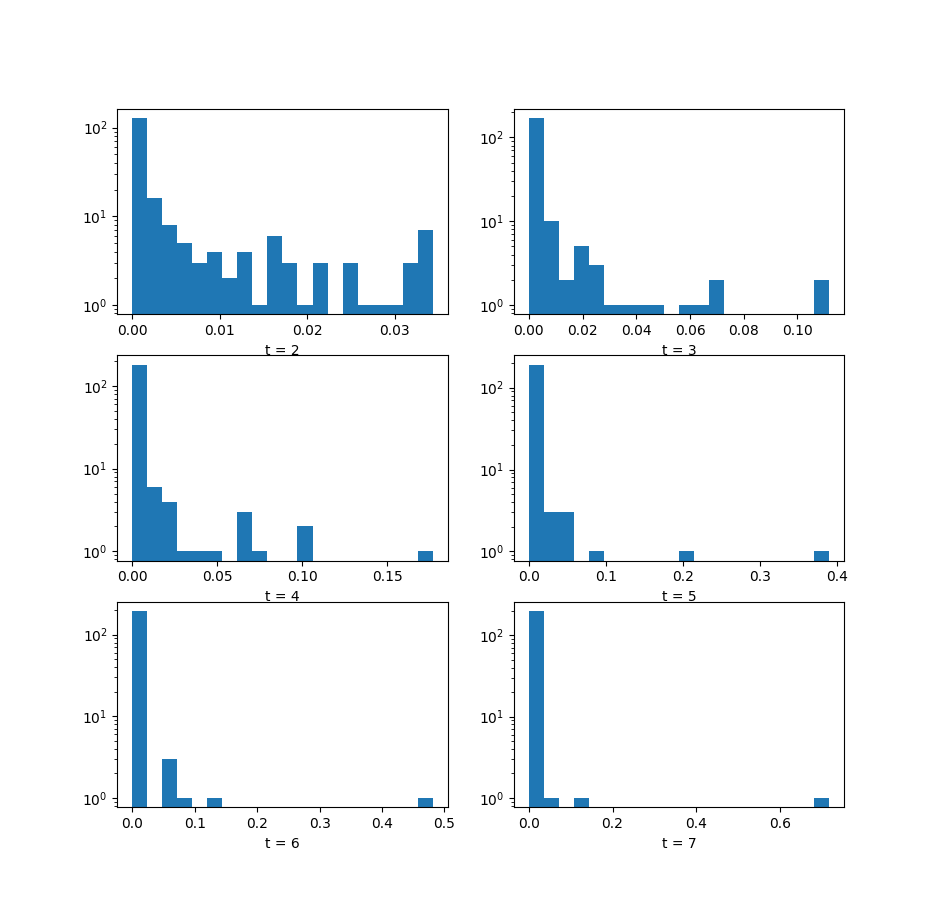
\includegraphics[width=1.3\textwidth]{figures/Figure_weights.png}
  }
  \caption{A histogram of 200 weights after just a few
    iterations. Almost all the weights are zero at $k = 7$ which
    demonstrates the degeneracy of the particles.}
  \label{fig:weights}
\end{figure}

\section*{Resampling}
We are going to present two resampling strategies in this section. The
overall goal of all resampling methods is to remove particles with
negligible weights with a high probability and replicate those with
high weights. After resampling, the future particles are more
concentrated in domains of higher posterior probability, which entails
improved estimates. It can, of course, happen that a particle with a
low weight at time $t$ has a high weight at time $t+1$, in which case
resampling could be wasteful. It should also be mentioned that if
particles have (unnormalised) weights with a small variance,
resampling might be unnecessary. This is discussed briefly at the end
of this section. As above, we denote by
$\{ x^{(i)}, w^{(i)} \}_{1 \le i \le N}$ the set of particles with
their associated weights at some time $k$ (which is omitted in the
notation). We assume that the weights have already been normalised,
i.\,e.\ $\sum_i w^{(i)} = 1$. We further denote by
$\{ \tilde{x}^{(i)}, \tilde{w}^{(i)} \}_{1 \le i \le N}$ the particles
and weights after resampling took place. We require the particles
$\tilde{x}^{(i)}$ to be weighted equally which implies, since we also
require the weights to be normalised, that $\tilde{w}^{(i)} = 1/N$.

The use of resampling to improve importance sampling was originally
introduced by Gordon et al, see~\cite{gordon}, laying the ground for
Particle filters and SMC methods in general. The resampling methods
presented here are two of the most popular amongst the literature,
see~\cite{douc}.  The most simple resampling strategy, called
\emph{multinomial resampling} is not discussed here due to its poor
performance compared to other techniques. It only is mentioned because
it is the method introduced by Gordon et al. in~\cite{gordon} as part
of the\emph{ bootstrap filter}, that uses the prior as the proposal
density (c.\,f.\ Examples~\ref{ex:1} and~\ref{ex:lv1}).

Both the methods presented in the following are based on drawing
samples from the point mass distribution
$\sum_{j=1}^N w^{(j)} \delta_{X^{(j)}}$. In practice, this is achieved
by repeated uses of the inversion method, which itself uses the
empirical cumulative distribution function (cdf) associated with the
weights. This is based on the following fact:

\textbf{Claim.}\quad If $U$ is a uniform random variable on $(0,1]$
then $X = F^{-1}(U)$ has distribution $F$, where $F$ is the cumulative
distribution function of $X$ and
$F^{-1}(t) = \min \{ x \mid F(x) = t \}$ is the inverse cdf.

\textbf{Proof.}\quad Let $U \sim \mathcal{U} (0,1]$. Then
\begin{align*}
  P(F^{-1}(U) \le x) &= P(\min \{x \mid F(x) = U \} \le x ) && \text{(definition of $F^{-1}$)} \\
                     &= P(U \le F(x)) \\
                     &= F(x) && \text{(definition of distribution of $U$)}\,.
\end{align*}
\hfill$\square$

The inversion method can be explained visually as follows. We plot the
empirical cdf of the weights and sample from
$U \sim \mathcal{U}(0,1]$. We denote the actual value of the sample by
$u$. We then draw a horizontal line from the coordinate $(0,u)$ to the
right until it intersects one of the bars, see
Figure~\ref{fig:ecdf}. The index of the bar that is intersected
determines the new sample.

\begin{figure}[htpb]
  \centering 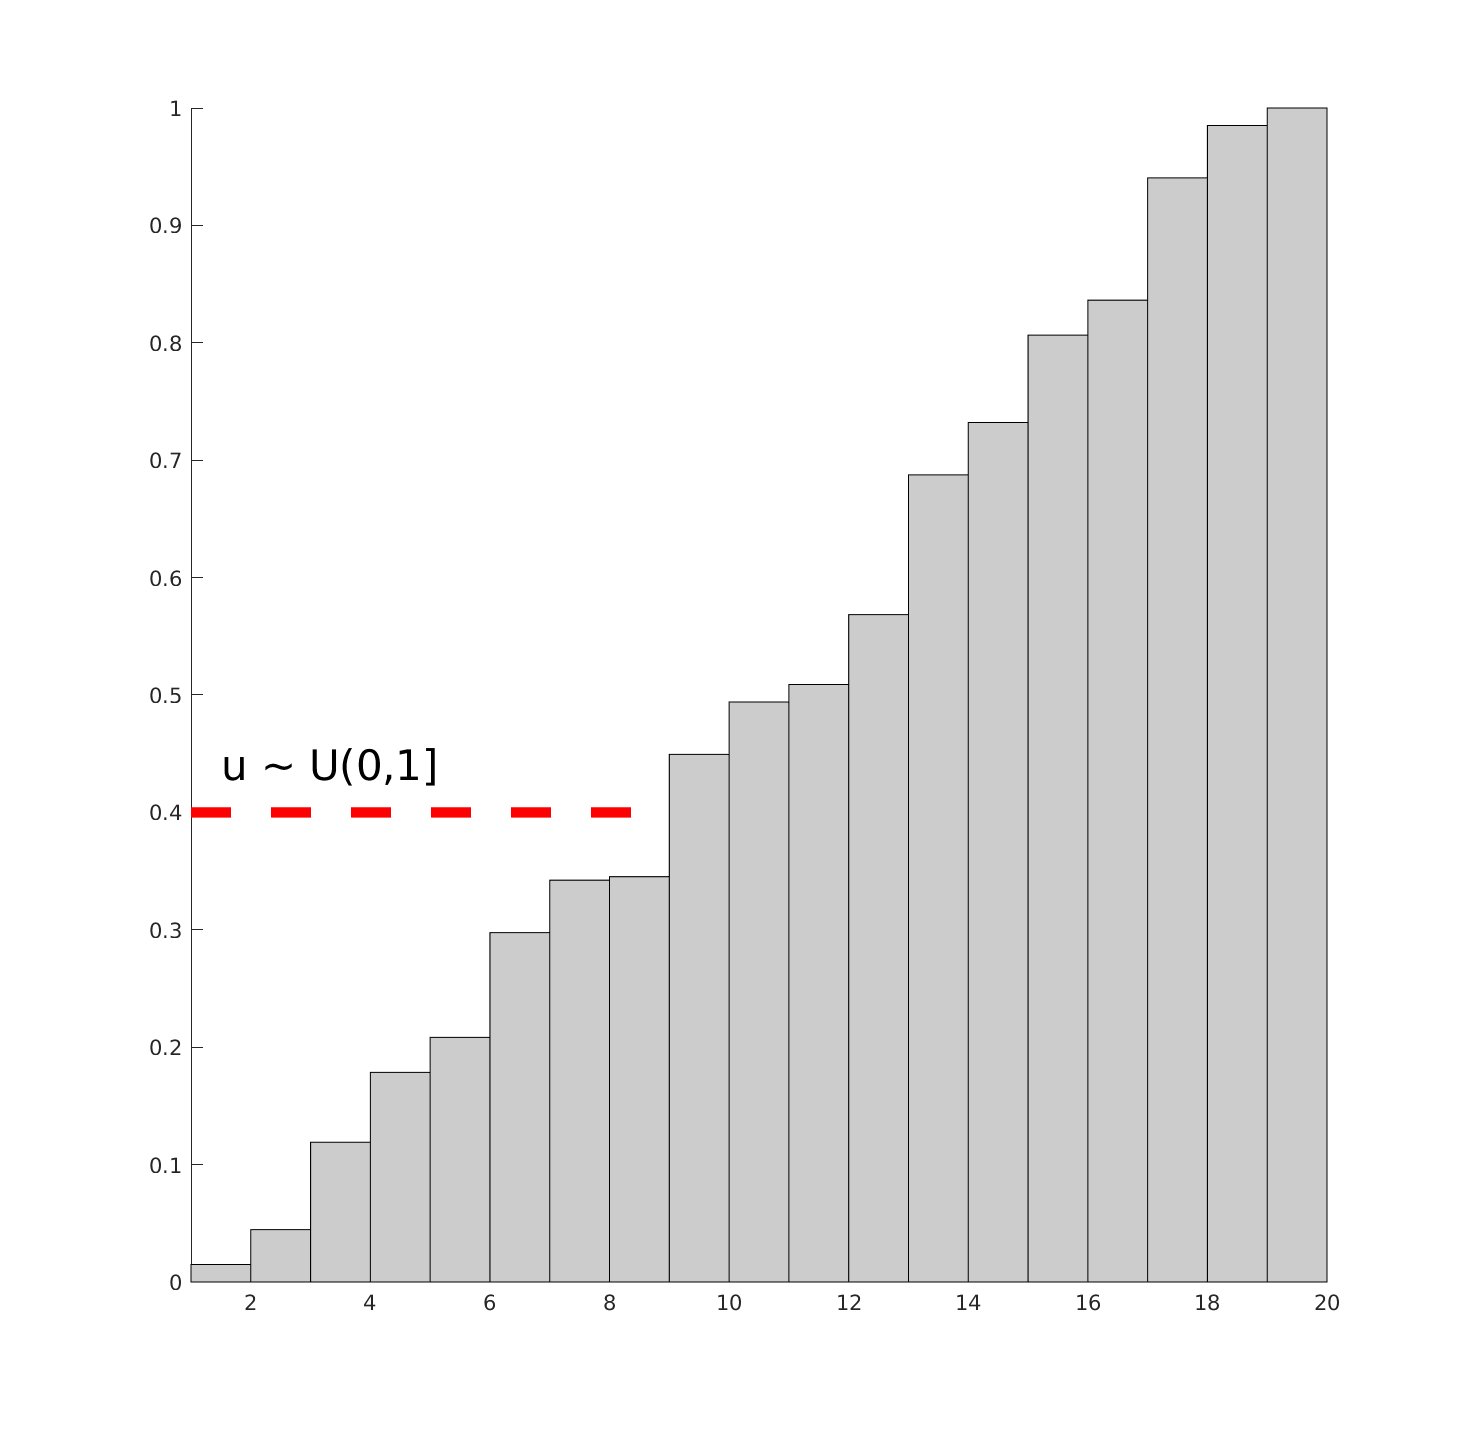
\includegraphics[width=\textwidth]{figures/ecdf.png}
  \caption{Visualisation of the inversion method. The bars represent
    the empirical cumulative distribution function associated with a
    set of 19 weights. The red line is horizontally drawn from the
    value of $u$ at the vertical axis until it ``hits'' a bar. The
    index of the bar yields the generated sample (in this case the new
    sample is therefore 9). }
  \label{fig:ecdf}
\end{figure}

In our case, we do not draw just one sample $U$ but we generate $N$
different samples $\{U_i\}_{1 \le i \le N}$ in such a way that they
are sorted in ascending order. For every of these samples (from lowest
to highest) we look for the intersected bar and add its index to a
list. This list then corresponds to the indices of the particles that
should be resampled. Consider the following example: Suppose we had
five particles and the list of indices after the resampling reads
$\{1,3,4,4,5\}$. Then, particles $X^{(1)},X^{(3)},X^{(5)}$ should be
resampled, particle $X^{(4)}$ should even be duplicated. Particle
$X^{(2)}$, however, will be dropped. In other words, the particles
after the resampling are
\begin{gather*}
  \tilde{X}^{(1)}=X^{(1)},\ \tilde{X}^{(2)}=X^{(3)},\ \tilde{X}^{(3)}=X^{(4)},\\
  \tilde{X}^{(4)}=X^{(4)},\ \tilde{X}^{(5)}=X^{(5)}\,.
\end{gather*}

The two strategies presented in the following only differ in the way
the $U_i$s are generated. We summarise the results in
Algorithm~\ref{alg:resampling}.

\begin{algorithm}[htpb]
  \SetAlgoLined \KwData{$N$ samples $U_i \sim \mathcal{U}(0, 1]$
    sorted in ascending order;\ list of weights} \KwResult{List of
    indices $I$ that represent that particles to be resampled} $C$ =
  \texttt{cumsum}(weights) \tcp*{Generate the empirical cdf as list of
    cumulated sums} $I$ = zeros(N)\; $i,j = 0$\; \While{$i < N$}{
    \eIf(\tcp*[h]{Found intersecting bar}){$U_i < C_j$}{ $I_i = j$\;
      $i = i+1$\; } { $j = j + 1$\; } }
  \caption{Resampling using the empirical cdf}\label{alg:resampling}
\end{algorithm}

Here, the function \texttt{cumsum} is assumed to work in the same way
as, for example, MATLAB's or NumPy's \texttt{cumsum} function. That
is, \texttt{cumsum([1,2,3,4])} should return \texttt{[1,3,6,10]}.

\subsection*{Systematic Resampling}
This algorithm separates the sample space into $N$ divisions. One
random offset, drawn from a $\mathcal{U}[0, 1)$ distribution, is used
to choose where to sample from for all divisions. This guarantees that
every sample is exactly $1/N$ apart.

In other words, the $U_i$s are generated by sampling
$\tilde{U} \sim \mathcal{U}[0, 1)$ and defining
\[
  U_i = \frac{\tilde{U} + i-1}{N} \quad \text{for } i = 1, \dotsc, N
  \,.
\]

\subsection*{Stratified Resampling}
This algorithm is similar to the previous one, its aim is to make
selections relatively uniformly across the particles. We start by
partitioning the $(0,1]$ interval into $N$ disjoint sets,
$(0,1] = (0, 1/N] \cup (1/N, 2/N] \cup \dotsm \cup ((N-1)/N, 1]$. The
$U_i$s are then drawn independently in each of the sub-intervals:
\[
  U_i \sim \mathcal{U}((i-1)/N, i/N]\,.
\]

We mentioned earlier that resampling might be unnecessary if the
weights are sufficiently uniform and we would like to have a criterion
allowing us to check whether resampling should be performed. To that
end the effective sampling size ($ESS$) is often used which can be
estimated using
\begin{equation}
  \label{eq:ESS}
  ESS \approx {\left( \sum_{i=1}^N {\left( w_t^{(i)} \right)}^2
    \right)}^{-1} \,,
\end{equation}
where the weights $w_t^{(i)}$ are assumed to be already normalised
(for more details, see~\cite[179]{arulampalam}). If the variance of
the weights is maximal, i.\,e.\ if all but one of the weights are
zero, the value of $ESS$ is 1. If, however, the weights all have the
same value $w_t^{(i)} = 1/N$ the value of $ESS$ is $N$, since
\[
  {\left( \sum_{i=1}^N {\left( \frac{1}{N} \right)}^2 \right)}^{-1} =
  {\left( N \frac{1}{N^2} \right)}^{-1} = N \,.
\]
Therefore, we will only resample if $ESS$ is below a certain
threshold, e.\,g.\ $N/2$.

We have now gathered everything we need to implement a particle
filter, since essentially particle filters are simply a combination of
sequential importance sampling and some resampling
strategies. Therefore, sometimes these methods are also called
as\emph{Sequential Importance Sampling with Resampling} abbreviated by
SIS/R.
%%% Local Variables:
%%% mode: latex
%%% TeX-master: "../main"  
%%% End:
